\documentclass{article}

% set font encoding for PDFLaTeX or XeLaTeX
\usepackage{ifxetex}
\ifxetex
  \usepackage{fontspec}
\else
  \usepackage[T1]{fontenc}
  \usepackage[utf8]{inputenc}
  \usepackage{lmodern}
  \usepackage{graphicx}
  \usepackage{siunitx}
  \usepackage{amsmath}
  \usepackage{float}
\fi

% used in maketitle
\usepackage[left=3cm,right=3cm,top=3cm,bottom=3cm]{geometry}
\title{Actividad 8}
\author{Luis Aarón Cerón Ramírez}

% Enable SageTeX to run SageMath code right inside this LaTeX file.
% documentation: http://mirrors.ctan.org/macros/latex/contrib/sagetex/sagetexpackage.pdf
% \usepackage{sagetex}

\begin{document}
\maketitle
El oscilador de Van de Pol es un oscilador con amortiguamiento no lineal, que esta dado por la ecuación diferencial de segundo orden
\begin{displaymath}
\frac{d^2x}{dt^2}-\mu(1-x^2)\frac{dx}{dt}+x=0
\end{displaymath}
\newline
donde x es la coordenada de posición(la cual es función del tiempo), y $\mu$ es un parámetro escalar que indica la no linealidad y fuerza del amortiguamiento.

\section{Historia}
Este oscilador fue propuesto originalmente por el físico e ingeniero electrico holandes Balthasar Van der Pol en 1920, cuando este se encontraba trabajando para la compañia Phillips.

\section{Forma en dos dimensiones}
Al usar el teorema de Liénard se puede probar que el sistema tiene un limite cíclico. Aplicando la transformación $y=x-x^3/3-\dot x/\mu$, por lo que el oscilador de Van der Pol se puede escribir como en la forma de dos dimensiones:

$\dot x=\mu(x-\frac{x^3}{3}-y)$

$\dot y= \frac{x}{\mu}$

\section{Resultados para el oscilador no forzado}
Dos interesantes regímes para el oscilador no forzado son:
Cuando $\mu$= 0, no hay amortiguamiento por lo que la ecuación se convierte en
\newline
$\frac{d^2x}{dt^2}+x=0$
\newline
La cual es la forma para oscilador armoníco simple, y siempre hay conservación de la materia. Cuado $\mu$ es mayor que cero, el sistema entrara en un limite cíclico. Cerca del origen x=$\dot x$= 0, el sistema es inestable, y lejos del origen el sistema es amortiguado. Este oscilador no tiene solución analítica exacta.

\section{Oscilador de Van der Pol forzado}
El oscilador de Van der Pol agrega a la expresión original y agrega una función de dirección $A\sin(\omega t)$ dando la forma:
\newline
$\frac{d^2x}{dt^2}-\mu(1-x^2)\frac{dx}{dt}+x-A\sin(\omega t)=0$
\newline
donde A es la amplitud ó desplazamiento de la función de onda y $\omega$ es la velocidad angular.

\section{Resultados}
La actividad consistió en recrear las imágenes de la pagina de wikipedia, por lo que se anexan las imagénes en esta sección.

\begin{figure}[h]
\centering
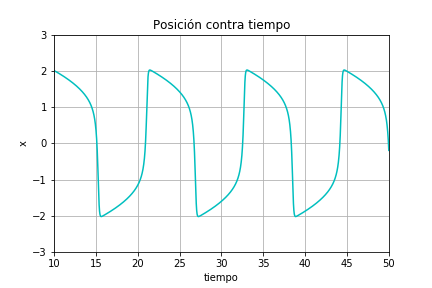
\includegraphics[scale=0.59]{Posicion_contra_tiempo.png}
\end{figure}

\begin{figure}[h]
\centering
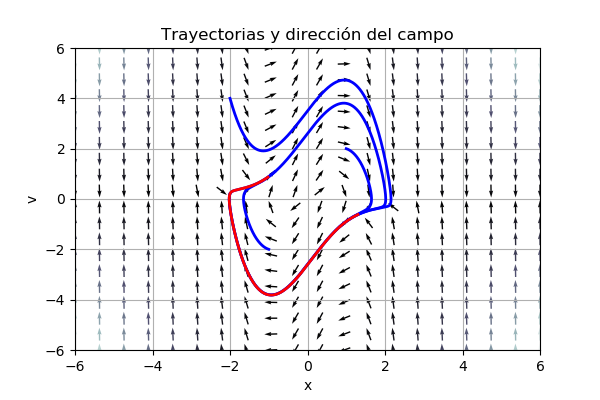
\includegraphics[scale=0.59]{FasesCondiciones.png}
\end{figure}

\begin{figure}[h]
\centering
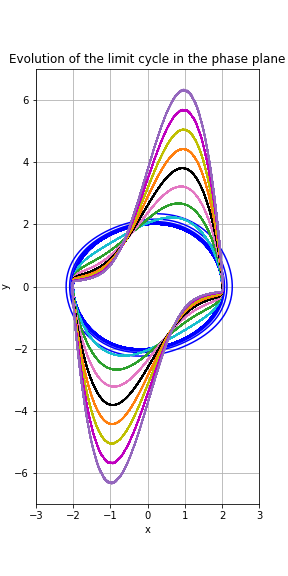
\includegraphics[scale=0.35]{Image2.png}
\end{figure}

\section{Conclusión}
Como ya se ha mencionado en los trabajos anteriores, se puede observar la importancia de estas herramientas al análisis de situaciones físicas, lo que ayuda a una mejor compresión sobre el comportamiento de los modelos lo que ayuda una mejor compresión n el estudio de estos modelos.

\section{Apéndice}
Este ejercicio pareciera similar al desarrollado en las actividades 6 y 7. ¿Qué aprendiste nuevo?
\newline
A programar un nuevo modelo asi como las implicaciones que este modelo tiene.
\newline
¿Qué fue lo que más te llamó la atención del oscilador de Van der Pol?
\newline
Las grafícas que se pudieron recrear y observar el comportamiento que estas tenian y compararlas con las actividades pasadas y ver las diferencias pues en los tres casos eran osciladores con características distintas.
\newline
Has escuchado ya hablar de caos. ¿Por qué sería importante estudiar este oscilador?
\newline
Si he escuchado, tengo entendido que son modelos que se encuentran en muchos casos fisicos como el pendulo doble
\newline
¿Qué mejorarías en esta actividad?
\newline
Mas fuentes para consultar la información
\newline
¿Algún comentario adicional antes de dejar de trabajar en Jupyter con Python?
\newline
No por el momento
\newline
Cerramos la parte de trabajo con Python ¿Que te ha parecido?
\newline
Me parecio que el uso de jupyter sera muy importante en los trabajos que siguen pues facilita de gran manera el trabajo con calculo asi como la graficación.

\end{document}
